\documentclass[10pt]{article}

%This is the minimal setup required to render the flag
\usepackage[paperwidth=144cm, paperheight=72cm, top=0cm, bottom=0cm, left=0cm, right=0cm]{geometry}
%Paper width is set to 144cm by 72cm to match the DPRK Government-specified aspect ratio (2:1)
\usepackage{tikz}
%\usepackage[dvipsnames]{xcolor} % Optional unless you want to use colors pre-defined by the xcolor package

% DPRK Government-specified colors for the flag
\definecolor{dprkred}{HTML}{ED1C27}
\definecolor{dprkblue}{HTML}{024FA2}
\definecolor{dprkwhite}{HTML}{FFFFFF}

% Other government specifications include:
% Blue stripe width is 1/12 flag width, here it is 12cm
% White stripe width is 1/72 flag width, here it is 2cm
% Red stripe width is 11/36 flag width, here it is 44cm
% Center of star (and circle) is 1/3 flag width (here it is 48cm) from left edge of flag
% Diameter of circle is 2/9 flag width, here it is 32cm
% Diameter of star is 31/144 flag width, here it is 31cm

%Source: https://commons.wikimedia.org/wiki/File:Flag_of_North_Korea_(Construction_sheet).svg

%Created by Senan Sekhon, August 5, 2021

\begin{document}

\begin{center} %Optional, but helps to tidy up the layout
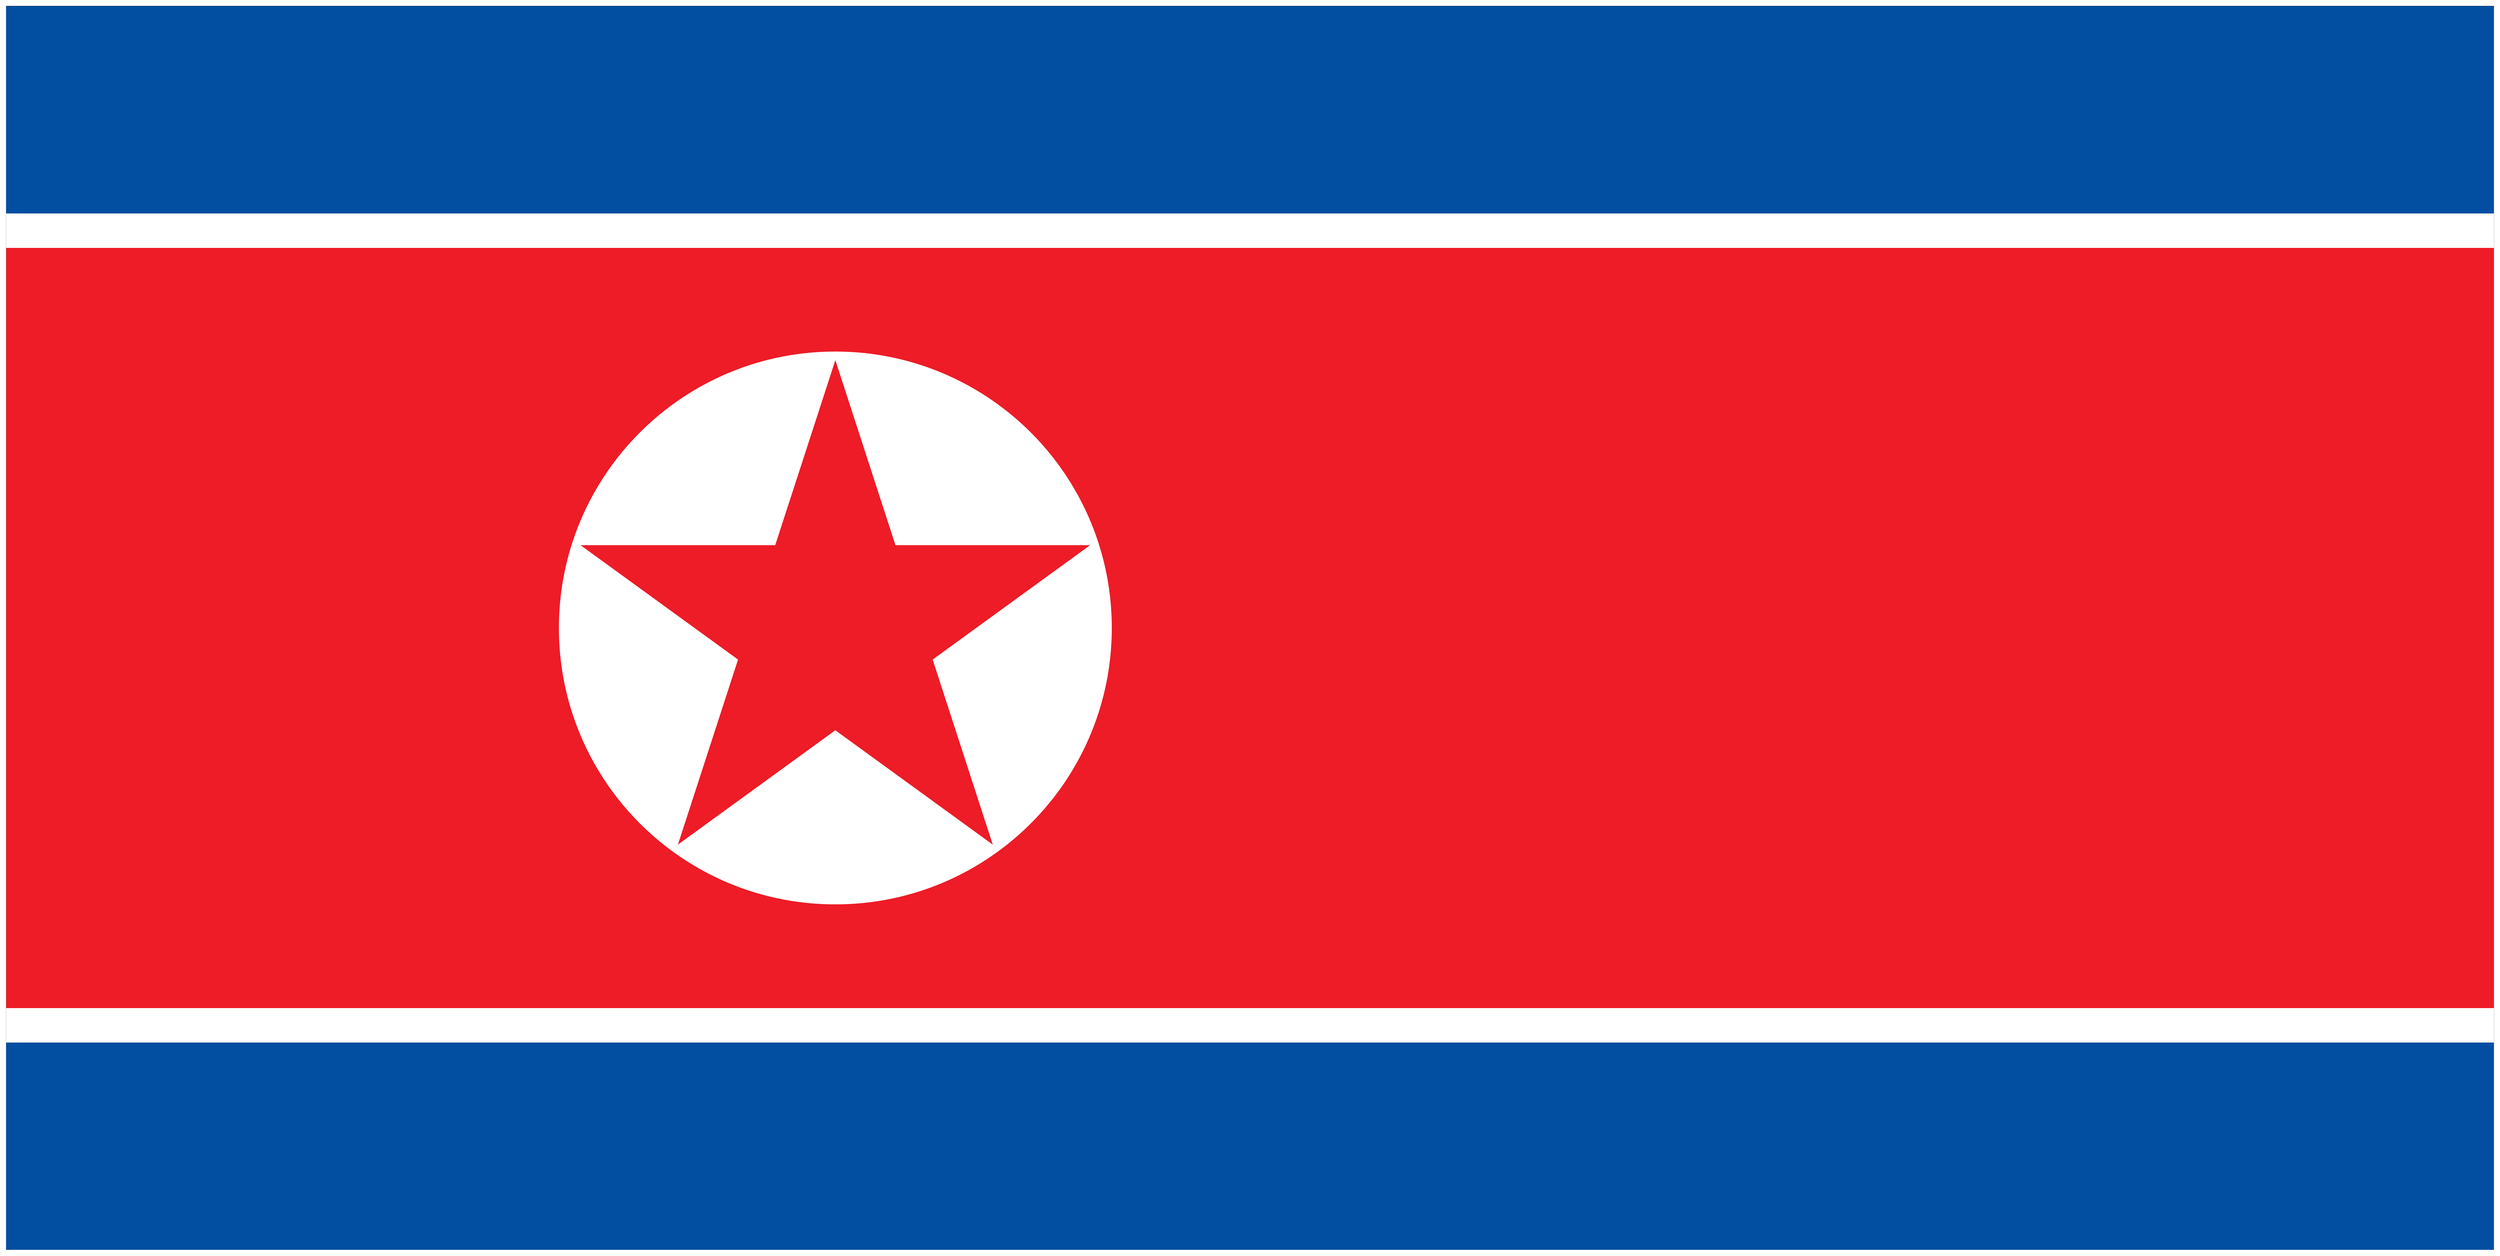
\begin{tikzpicture}[scale=1] %Scale must be changed to make the flag fit on letter/A4 paper (scale=1 produces a 144cm by 72cm flag)
\clip (-72,-36) rectangle (72,36); %Optional, crops the flag to the correct size
\draw[-] (-72,-36) rectangle (72,36); %Optional, draws a border around the flag
\fill[dprkblue] (-72,24) rectangle (72,36); %Top blue stripe
\fill[dprkwhite] (-72,22) rectangle (72,24); %Top white stripe
\fill[dprkred] (-72,-22) rectangle (72,22); %Red stripe
\fill[dprkwhite] (-72,-24) rectangle (72,-22); %Bottom white stripe
\fill[dprkblue] (-72,-36) rectangle (72,-24); %Bottom blue stripe
\begin{scope}[shift={(-24,0)}] %Circle and star
\fill[dprkwhite] (0,0) circle (16); %White circle
\fill[dprkred] (90:31/2)--(54:{31/4*(3-sqrt(5))})--(18:31/2)--(-18:{31/4*(3-sqrt(5))})--(-54:31/2)--(-90:{31/4*(3-sqrt(5))})--(-126:31/2)--(-162:{31/4*(3-sqrt(5))})--(-198:31/2)--(-234:{31/4*(3-sqrt(5))})--cycle; %Red star
\end{scope}
\end{tikzpicture}
\end{center}

\end{document}